\documentclass[12pt,english,oneside,letterpaper]{report}
%\documentclass{article}
\usepackage[utf8]{inputenc}
\usepackage{amsmath}
\usepackage{subcaption}
\usepackage{pdfpages}
\usepackage{placeins}
%\usepackage[thinlines]{easytable}
%\pgfplotset{compat=1.8}
\usepackage{setspace}
\usepackage{cite}
\usepackage{graphicx}
\graphicspath{{Figures/}}
\usepackage{fancyhdr}
\pagestyle{headings}
\usepackage{refstyle}
\usepackage{subfiles}
%\usepackage{comment}
\usepackage{titlesec}
\titleformat{\chapter}[hang]{\bf\huge}{\thechapter}{2pc}{}
\usepackage{titletoc}
\usepackage{tocloft}
\usepackage{hyperref}
%\usepackage{comment}
\usepackage{cleveref}
%\usepackage{cleveref}
\usepackage{setspace}
\usepackage[nottoc]{tocbibind}
%\usepackage{afterpage}
%\usepackage{titlesec}

\titleformat*{\chapter}{\LARGE\bfseries}
\pagenumbering{roman}

\pagestyle{plain}
\usepackage{morefloats}
\usepackage{subfiles}
\usepackage{blindtext}
\usepackage{amssymb,enumitem}
\usepackage{amsmath}
\usepackage[ruled ]{algorithm2e}
\usepackage{verbatim}
\usepackage{float}
\usepackage{overpic}
\usepackage{array}

\usepackage{blindtext}
\usepackage{scrextend}
\RequirePackage[left=3.25cm,right=2.5cm,top=2.5cm,bottom=2.5cm]{geometry}

\renewcommand{\baselinestretch}{1.6}



\newenvironment{dedication}
  {\clearpage           % we want a new page
   \thispagestyle{empty}% no header and footer
   \vspace*{\stretch{1}}% some space at the top 
   \itshape             % the text is in italics
   \centering          % flush to the right margin
  }
  {\par % end the paragraph
   \vspace{\stretch{1}} % space at bottom is three times that at the top
   \clearpage           % finish off the page
  }

\begin{document}

\author{Faisal Ameen Zaman}
\begin{titlepage}
\begin{center}
% \vspace*{0.2cm}
 {\huge \textbf{How To use Latex for Thesis Writing}}
\vspace*{0.2cm}
\begin{center}
{\Large {\textbf{Faisal Ameen Zaman}}} 
\end{center}
\vspace*{0.2cm}
\begin{center}
{ A thesis submitted to the Faculty of Graduate and Postdoctoral Affairs in partial fulfillment of the requirements for the degree of} 
\end{center}
\vspace*{0.2cm}
\begin{center}
{\Large {\textbf{Masters Of Applied Science}}} 
\end{center}
%\vspace*{0.2cm}
%\begin{center}
%{\Large {in}}
%\end{center}
%\vspace*{0.2cm}
\begin{center}
{ In Electrical and Computer Engineering} 
\end{center}
\vspace*{1.0cm}
\begin{center}
{Ottawa-Carleton Institute for Electrical and Computer Engineering\\
School of Electrical Engineering and Computer Science\\
University of Ottawa\\
Ottawa, Canada} 
\end{center}
%\vspace*{1.0cm}
\begin{center}
{ January 2017} 
\end{center}
\vspace*{1.0cm}

\begin{center}
{\textbf{\copyright \ 2017 Faisal Ameen Zaman}} 
\end{center}
\end{center}
\end{titlepage}



\chapter*{Abstract}
%VN Embedding\\
%SDN\\
%Metro Optical\\
%Edge Datacenter\\
%\vspace{-15mm}
\setcounter{page}{1}
\addcontentsline{toc}{chapter}{Abstract}
This is just an example of showing how to use latex for writing the Thesis. I was a master student at University of Ottawa and I found it very useful to write my thesis using Latex. I spent lot of time finding easy methods to perfrom certain things such as conisdering the documentclass as Report or book will give you more flexibility with the packages rather than going as an article, how to write an Algorithm, and How to include image to name a few. I prefer including images in PDF format as it gives clarity and sharpness while printing. I have left couple of images to see how to include pdf as images. I have tried my best to cover everything I know and learnt about latex in this document. Well one thing I have learnt from my research is that one technique optimal for one person is not optimal for another person.\par
Good Luck !! \par

\chapter*{Acknowledgement}
\addcontentsline{toc}{chapter}{Acknowledgement}
\vspace{-12mm}
This thesis would have remained a dream, had it not been for my Professor Ahmed karmouch. Whose unflinching confidence in my abilities metamorphosed my personality. ``Good, Better, Best. Never let it rest. Till your good is better and your better is best" - St. Jerome. The above quotation is the hallmark of my Professor's work ethics. He always insisted to bring out the best, with a great sense of accomplishment. I would like to express my deepest gratitude to Professor Ahmed karmouch.\par
I would like to express deepest appreciation and thankfulness to Dr. Abdallah Jarray. His attitude and genius continuously and convincingly through out the research work has enabled me to present this thesis. He inspired, guided and motivated me at all times of research work. I would not have imagined a better advisor and mentor.\par
My sincere thanks to Heli Amarasinghe, Venkatraman Balasubramanian and Wijay Ekanayake and other Lab colleagues, without their precious support, it would have not been possible to write this thesis. I am deeply indebted to my brother Mohammad Farooq Zaman for his moral support, encouragement and guidance. He has been a pillar of strength to me at all times. My sincere thanks to Hisham Veeran, Mudasser Noor, Yasir Noor, Fazal Noor and Mohammed Riyaz  for their moral support.\par
My thanks to University of Ottawa for giving me access the resources to carry out my research and write this thesis. I also thank my many friends for their moral support and guidance. I also thank all those who directly or indirectly helped me complete this challenging task.\par
``As we express our gratitude, we must never forget that the highest appreciation is not to utter words, but to live by them", - John F Kennedy. Sincere thanks to my parents, Rahat Jahan and Badruzzaman for their unconditional love and support.\par
\clearpage

\begin{dedication}
Dedicated ToVenkatraman and Heli
\end{dedication}
\let\cleardoublepage\clearpage
%\noindent\makebox[\linewidth]{\rule{\paperwidth}{0.4pt}}

\tableofcontents

\chapter*{List Of Acronyms}
\addcontentsline{toc}{chapter}{List Of Acronyms}
\begin{table}[H]

\begin{tabular}{ l  l}
\textbf{Acronym} & \textbf{Expansion}  \\
APEX & Capital Expenditure \\
CDC & Colorless Dimentionless Contentionless\\
\end{tabular}

\end{table}
\clearpage
%\chapter*{List of Table}
\listoffigures
%\chapter*{List of Figures}
\clearpage
\listoftables
\clearpage
%\begin{spacing}{1.5}

%\end{spacing}

%\tableofcontents

%\mainmatter
% Chapter 1
\chapter{Introduction}
\label{chap:one}
\pagenumbering{arabic}
This is Chapter 1.  Extend the number of chapters as you need.
I don't recommend including any images in chapter one but, It all depends on your prof. 
\section{Motivation}
\section{Thesis Objective}
\section{Contribution}
\section{Organization}

%\pagenumbering{arabic}


% Chapter 2
\chapter{Background and Related Works}
\label{chap:two}
\section{Objective}
I prefer using the PDF as images rather than Jpeg or 
\begin{figure}
\centering
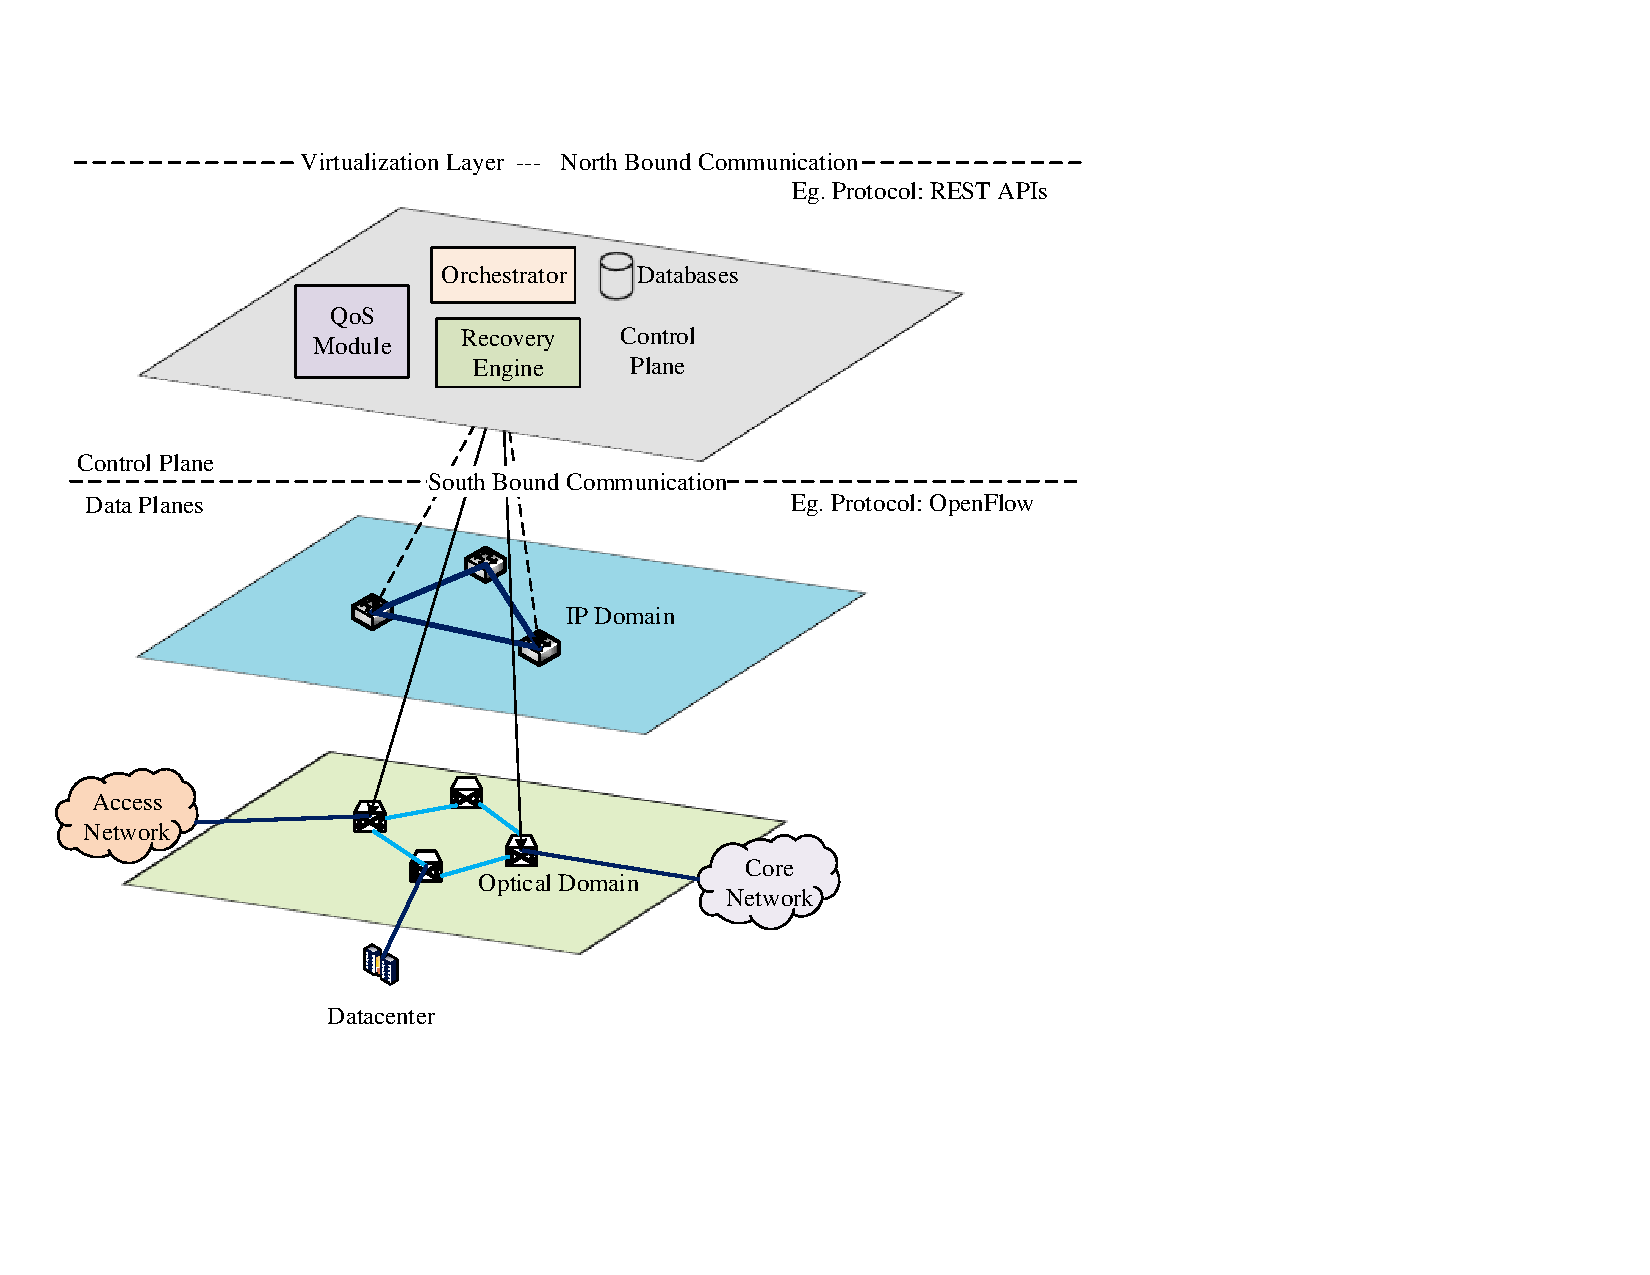
\includegraphics[clip, trim=0.4cm 4cm 9.5cm 2cm ,width=0.85\columnwidth]{General/Chapter2/sdnmon.pdf}
\caption{SDN-based for Metro Network}
\label{fig:sdnmon}
\end{figure}
VN embedding is an NP-hard problem; several approaches for solving this problem using SDN are discussed in the following section.\par
\subsection{Some related sections}

\section{Summary}
This is the summary section where you do the breifing of what ever you have explained earlier.

%\begin{comment}% Chapter 3
\chapter{Your Main Contribution Chapter one}
\label{chap:three}
\section{Objective}


\section{Overview of the Adapted Architecture for VN Embedding using SDN}

	\subsection{Problem Description} 
		The problem description if you have any mathamatical model.


\section{Mathematical Model Adapted for VN Embedding}
In this section I have shown the example of three ways to include equations in the latex.
\begin{equation}
 K_s = (H_s,L_s) 
\end{equation}
This equation is characterized by a set of substrate nodes $H_s$ and a set of links $L_s$.\\
The substrate node \textit{u} $\in H_s$, can be defined by:
\begin{equation}
u=\{R_u, S_u, G_u, C_u\}
\end{equation}
where, $R_u$, is the Memory, $S_u$ is the storage capacity, $G_u$ is the GPU, and $C_u$ is the CPU capacity of the node $u$.
The residual CPU, Memory, Storage and GPU capacity is given by,
$P^{r/s/g/c}_u(t)$ the available memory/RAM, storage, GPU, CPU capacity at time period $t$.
Hence, at any given time the available node capacity can be defined by a set 
\begin{equation}
Q_u = \{ P^r_u(t), P^s_u(t), P^c_u(t), P^g_u(t)\}
\end{equation}
A VN request can be represented as $K_v = (H_v, L_v)$ where, $H_v$ represents set of virtual nodes and $L_v$ represents directional Links.
The QoS requirement of a virtual node $a$ $\in H_v$ can be defined as:
\begin{equation}
(QoS)_a = (p_a^r, p_a^s, p_a^g, p_a^c)
\end{equation}
$P_a^{r/s/g/c} $ represents required RAM, Storage, GPU and CPU at a selected substrate node for processing the selected VN request. Similarly, for a virtual link $e \in L_v$, can be defined by a set:
\begin{equation}
(QoS)_e = (b_e, d_e)
\end{equation}
$b_e$ and $d_e$ define the minimum required bandwidth and delay for the selected virtual request respectively.
$x_a^u$ and $z_n$ are binary variables. $x_a^u$ is $1$ if a virtual node $a$ is assigned to substrate node $u$, 0 otherwise. Similarly, $z_n$ is a binary variable which is 1 if a virtual network request is accepted, 0 otherwise.\par
$Objective$ $Function:$
To increase the revenue by maintaining QoS requirement for VN requests, i.e., maximizing profit. Eq (6) defines the objective function.
 \begin{multline}
f_{objective} = \sum_{n \in N} \Bigg\{\sum_{e\in L_v; e=(sd)}  P_e^n *z_n - 
\sum_{ (u,v) \in H_s * H_s} x_s^u * x_d^v * (f_u + f_v + \sum_{l \in \pi(uv)}c_l * b_e)\Bigg\}
\end{multline}

The option align is good when you have to align multiple equations at certain point. In the given example I have aligned them at assignment operator or comparision operation point. I.e., LHS to RHS point.
\begin{align} 
\sum_{c \in C} \lambda_c &\leqslant W \quad &(\alpha_o) \label{eq:3} \\
\sum_{c \in C} \lambda_c * T_c(u) &\leqslant N_{ROADMs}(u) \quad &(\mu_u) \label{eq:4}\\
\sum_{c \in C} \lambda_c * a_c^n &\geqslant 1 ; u \in H_s ; n \in N. \quad &(\beta_u) \label{eq:5}
\end{align}

\section{Summary}
Summary goes here


% Chapter 5
\chapter{Implementation And Evaluation}
\label{chap:five}
\section{Objective}
While explaining figues using Latex I will always suggest you to use Labels for the images. The reason is you would not know where the images willl be located after compilation (unless you use `H' as an attribute, which is not advisable). So always use labels and use them as as `\\ref'  in the expalination in that way you will need not worry about the whereabouts of the images.
This chapter deals with providing the proof of concept for the architecture and formulation proposed in chapter 2 and chapter 3 respectively.  The Software used to perform simulation is explained. The solvers like Gurobi and CPLEX which adapted to solve the combinatorial problem are briefly shown. Finally, an in-depth inference on the obtained results is given. \par

\section{Implementation Methodology}

This is a simple Algorithm using the package algorithmic. It shows binpacking used in my thesis.
Hope this helps you.



\begin{algorithm}
\SetKwFunction{KwFn}{\textbf{BestPaths}}

\KwFn{$a_s,a_d,\pi_{u,v}$}\\
\Begin{
 \ForEach{path in $\pi_{u,v}$}{
     	\ForEach {Paths in $ \pi_{u,v}$ }{
		cost[]$\leftarrow$  Calcuate Cost of Each Cost\;
	}
            \ForEach {cost in cost[]}{
	    	$\Pi_{u,v}  \leftarrow $ Path with least cost in $\pi_{u,v}$\; 
	}
}Return{ \{$\Pi_{u,v}$, cost $\Pi_{u,v}$ \}}}

\SetKwFunction{KwB}{\textbf{BinPacking}}
\KwB{$\Pi_{u,v}$}\\
\Begin{
\ForEach {link in $\Pi_{u,v}$}{
  \ForEach{ Wavelength in link}{
      AvailableWavelength[] $\leftarrow $getWavelength(link)\;
	  }
}
\ForEach{ wavelength in AvailWavelength[]}{
	compare if all the Links in path $\Pi_{u,v}$ in \\ AvailWavelength[] has the wavelength available.\\
	\eIf { available wavelengths in path $\Pi_{u,v}$ is true for all links in it}{
			Return( Selected Wavelength)\\ 
			break\;
			}{Update
\\
			$\Pi_{u,v} \leftarrow$ BestPaths$(a_s,a_d,\pi_{u,v})$}
	\If { no path found in $(a_s, a_d,\pi_{u,v})$}{
			Return Embedding Not Possible\\
			Select New VN Request
			}
		      }
	Return ( Selected Wavelength)
 }
\caption{Selecting Links and Wavelegths for between the Substrate Nodes}
\label{algo:one}
\end{algorithm} 



\section{Discussion of Results}
\subsection{Definition of Metrics Used For the Evaluation}
Always Try to create images for gray scale. Because I had hard time converting all my results from color images to gray scale images at the end. And of-course no body wants to take print out in color.   The paths where I have included images is kind of long, but you can change the paths for your convinience. 
 \begin{figure}[H]
\centering
\frame{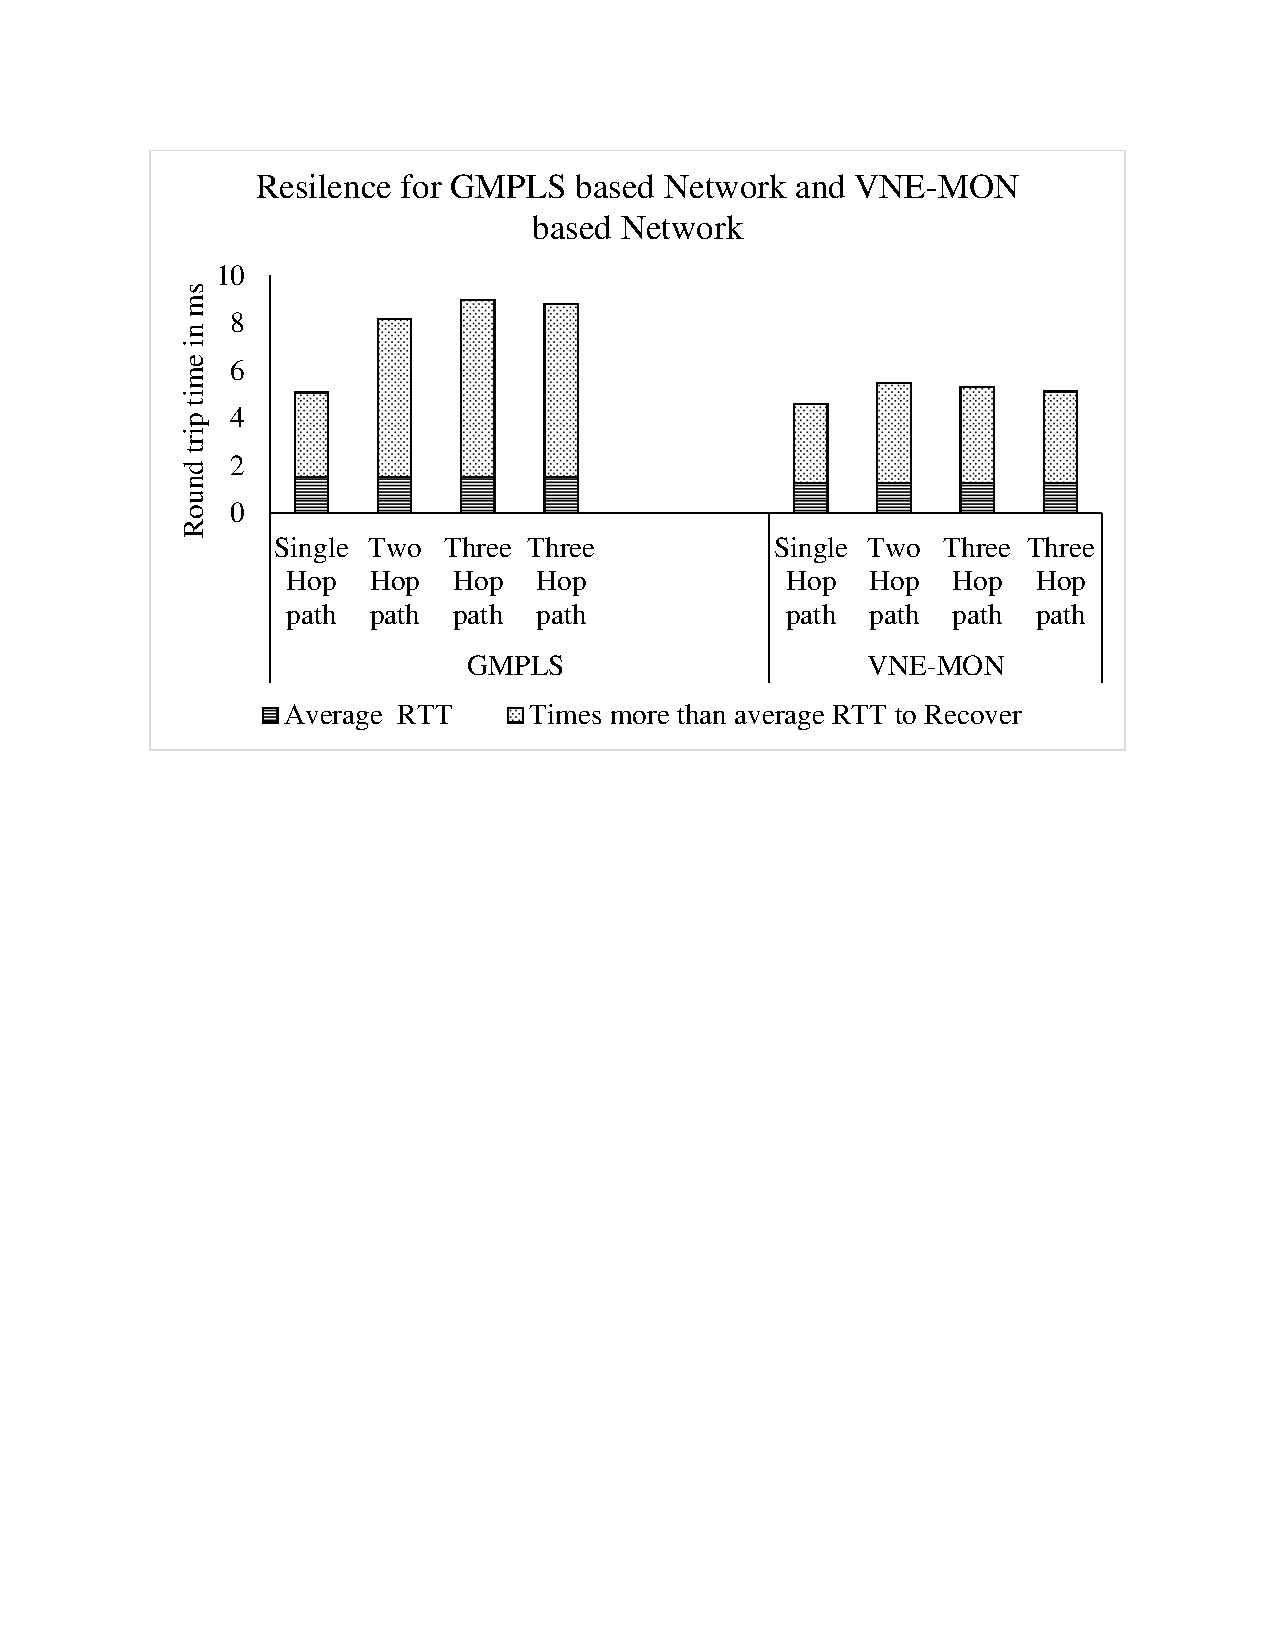
\includegraphics[clip, trim= 2.5cm 15.2cm 2.5cm 2.5cm,width=0.70\columnwidth]{Results/pdf/ResultsPDF/fourteen.pdf}}
\caption{ Cost vs. SRLG factor.}
\label{fig:before4}
\end{figure}

\section{Summary}
  


% Chapter 6
\chapter{Conclusion And Future Work}
\label{chap:six}
\section{Conclusion}

\section{Future Work}
\subsection{Proactive Determination of Controller Location Based on Traffic Predictability.}

\section*{Final Comments}
The star at the end of section will consider this section as a section but it won't include in the content section. This way you can avoid many trivial things to get included in the content and still be able to give the attributues of certain section or subsection or even a chapter. 
%\cite{one}
%\end{comment}
\begin{thebibliography}{9}

\bibitem{datacenteravailable}
Stacy Patterson et.al., \emph{``Serializability, not serial: concurrency control and availability in multi-datacenter datastores, "} Proceedings of the VLDB Endowment (PVLDB), 2012, Vol. 5, No. 11, pp. 1459-1470

\bibitem{SSF}
``Scalable Simulation Framework", Ssfnet.org, 2017. [Online]. Available: http://www.ssfnet.org/homePage.html. [Accessed: 23- Jan- 2017].
\end{thebibliography}

\end{document}